\documentclass{report}
\usepackage[margin=1in]{geometry} 
\usepackage{amsmath}
\usepackage[T1]{fontenc}          % change font encoding to T1
\usepackage{lmodern}  %better for visual on screen
\usepackage{graphicx}
\usepackage{float}

% Used for adding Matlab Algorithms
\RequirePackage{listings}
\RequirePackage[framed,numbered]{matlab-prettifier}

\begin{document}
\section*{lsr.m}
The function \textit{lsr.m} is a standalone matlab script that was written to perform least squares regression.  Matlab has built in functions \textit{lscov.m} for linear regression and \textit{nlinfit.m} for nonlinear regression. \textit{lsr.m} is intended to parallel the syntax of nlinfit, with the additional functionality to:
\begin{itemize}
	\item perform total least squares
	\item perform linear least squares
	\item automatically detect linearity of the modelfun using numerical Hessian
	\item input analytical Jacobians
	\item perform $\chi^2$ Goodness of fit test to determine the significance of the computed reference variance $\sigma_0^2$
	\item disable covariance matrix scaling
	\item add an estimate of the beta coefficients as observation equations
\end{itemize}
\clearpage
\section*{Example Usage (\textit{exampleLsr.m})}
\subsection*{Fit Unweighted 2D Data with Different Models}
\lstinputlisting[
label      = {alg:lsr2},
style      = Matlab-editor,
basicstyle = \mlttfamily,
firstline  = 2,
lastline   = 22,
firstnumber= 2
]{../exampleLsr.m}
\subsection{Fit a Plane to 3D data}

\begin{figure}[H]
	\centering
	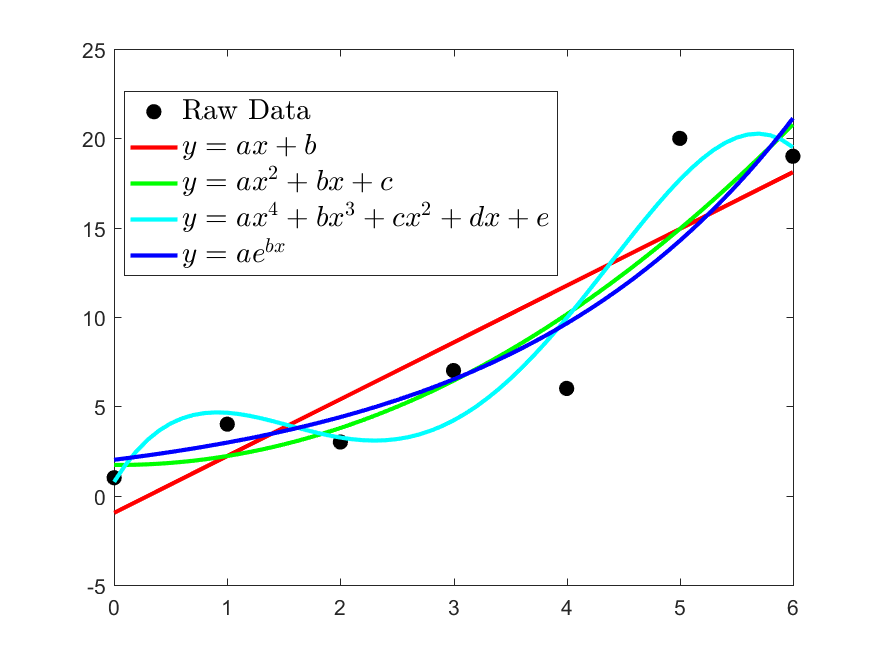
\includegraphics[height = 4in]{basicUsage}
\end{figure}

\subsection*{Sin Wave with known period}
\[y = a\sin(\dfrac{2\pi}{T}x+\phi)\]
\clearpage
\subsection*{2D Conformal Coordinate Transformation}
The 2D Conformal equations are:
\begin{align*}
X &= (S\cos(\theta))x - (S\sin(\theta))y + T_x \\
Y &= (S\sin(\theta))x + (S\cos(\theta))y + T_y
\end{align*}

\noindent
By substituting: 

\begin{align*}
a &= S\cos(\theta) \\
b &= S\sin(\theta)
\end{align*}
Where:

\begin{align*}
\theta &= \tan^{-1}(\dfrac{b}{a}) \\
S &= \dfrac{a}{\cos(\theta)}
\end{align*}

\noindent
The observation equations become:

\begin{align*}
F: \hspace{1cm} X &= ax - by + T_x \\
G: \hspace{1cm} Y &= bx + ay + T_y
\end{align*}

\noindent
Note that every $(X,Y)\rightarrow(x,y)$ correspondence produces 2 observation equations.

\lstinputlisting[
label      = {alg:lsr2},
style      = Matlab-editor,
basicstyle = \mlttfamily,
firstline  = 34,
lastline   = 40,
firstnumber= 34
]{../exampleLsr.m}

\lstinputlisting[
label      = {alg:lsr2},
style      = Matlab-editor,
basicstyle = \mlttfamily,
firstline  = 12,
lastline   = 30,
firstnumber= 12
]{../exampleLsr.m}




\section*{Equations Used}
\subsection*{Linear Least Squares}

\subsection*{Nonlinear Least Squares}

\subsection*{Total Least Squares}

\subsection*{Robust Least Squares (Iterative Re-weighted)}

\clearpage

\lstinputlisting[
label      = {alg:lsr},
style      = Matlab-editor,
basicstyle = \mlttfamily,
firstline  = 1,
lastline   = 48,
firstnumber= 1
]{../lsr.m}

\subsection*{Variable Definitions}
	\begin{align*}
		m & = \text{Number of Observation Equations} \\
		n & = \text{Number of Unknowns} \\
		p & = \text{Number of Observation Equations per Observation} \\
		q & = \text{Number of Predictor Variables per Observation}\\
		\beta &= \text{Estimated Regression Coefficients} \\
		x &= \text{Predictor Variables} \\
		y &= \text{Response Variables} \\
		V &= \text{Residuals} \\
		V_{eq} &= \text{Equivalent Residuals (TLS)} \\
		F(\beta,x) &= \text{Observation Equation} \\
		w &= \text{Vector of Weights for each observation} \\
		W &= \text{Weight Matrix} \\
		W_{eq} &= \text{Equivalent Weight Matrix (TLS)} \\
		\Sigma_{xx} &= \text{Covariance Matrix of Predictor Variables} \\
		\Sigma_{yy} &= \text{Covariance Matrix of Response Variables} \\
		\Sigma_{\beta \beta} &= \text{Covariance Matrix of Estimated Regression Coefficients} \\
		\sigma_0^2 &= \text{Computed Reference Variance} \\
		Q &= \text{Cofactor Matrix} \\
		\sigma_\beta &= \text{Standard Deviation of Estimated Regression Coefficients } \\
		\hat{y} &= \text{Predicted Response Variables} \\
		R^2 &= \text{model skill (Does not apply to nonlinear equations)} \\
		RMSE &= \text{Root Mean Square Error} \\
	\end{align*}
		
	Equations:
	\begin{align*}
		y &= F(\beta,x) \\ 
	\end{align*}
	Linear Least Squares Equations:
	\begin{align*}
		WA\beta &= y \\
		\hat{\beta} &= (A^TWA)^{-1}WA^Ty + WV\\
	\end{align*}
	NonLinear Least Squares Equations:
	\begin{align*}
		WJ_{y\beta}\Delta\beta &= K = y - F(x,\beta) + WV \\
		\hat{\Delta\beta} &= (J_{y\beta}^TWJ_{y\beta})^{-1}WJ_{y\beta}^TK \\
	\end{align*}
	Total Least Squares Equations:
	\begin{align*}
		J_{yx}V + J_{y\beta}\Delta\beta &= K = y - F(\beta,x) + V_{eq} \\
		W_{eq} &= (J_{yx}\Sigma_{xx}J_{yx}^T)^{-1} \\
		\hat{\Delta\beta} &= (J_{y\beta}^TW_{eq}J_{y\beta})^{-1}W_{eq}J_{y\beta}^TK \\
	\end{align*}
	Robust Least Squares Equations:
	\begin{align*}
		\text{Hat Matrix: } H &= J_{y\beta} (J_{y\beta}^TJ_{y\beta})^{-1} J_{y\beta} \\
		\text{Leverages: }h &= diag(H) \\
		\text{Adjusted Residuals: }R_{adj} &= R*sqrt(h) \\
		\text{Ensure minimum residuals: }R_{adj} &= max(1e-6,R{adj}) \\
		\text{Estimated std (Median Absolute Residuals): }\hat{\sigma_{R_{adj}}} &= MAD(R_{adj})/0.6745 \\
		\text{Normalized Residuals: }R_{norm} &= R_{adj}/(RobustTune * {\sigma_{R_{adj}}}) \\
		\text{Weight Vector: }W &= RobustWgtFun(R_{norm}) \\
	\end{align*}
\end{document}